\documentclass[11pt, a4paper]{article}
\usepackage[a4paper, margin=2.5cm]{geometry}
\usepackage{iftex}
\usepackage{graphicx}
\ifPDFTeX
    \usepackage[english]{babel}
\else
    \usepackage{fontspec}
    \usepackage[english, bidi=basic, provide=*]{babel}
    \babelprovide[import, onchar=ids fonts]{english}
    \babelfont{rm}{Noto Sans}
\fi
\usepackage{amsmath}
\usepackage{booktabs}
\usepackage{array}
\usepackage{xcolor}
\usepackage{hyperref}

\hypersetup{
    colorlinks=true,
    linkcolor=blue,
    urlcolor=blue,
    pdftitle={Standard and Non-Standard Convolutional Neural Networks on the MAMe Dataset}
}

\newcommand{\pair}[2]{\author{#1 \and #2}}
\newcommand{\todo}[1]{\textbf{\textcolor{red}{[TODO: #1]}}}

\title{Deep Learning Lab 1: Standard and Non-Standard CNNs on the MAMe Dataset}
\pair{Benjamin Krief}{Milan Van den Eede}
\date{\today}

\begin{document}
\maketitle

\section{Experimental Setup and Methodology}

To evaluate the performance of standard Deep Convolutional Neural Networks (CNNs) trained from scratch on fine-grained artwork medium classification, we use the $256 \times 256$ RGB version of the Museum Art Medium (MAMe) dataset. The dataset aggregates 37,407 artworks across 29 medium classes from three major museums and is partitioned into a balanced training set of 20,300 images (700 per class), a balanced validation set of 1,450 images (50 per class), and an unbalanced test set of 15,657 images.

All images are loaded at their native $256 \times 256$ resolution and normalized to the $[0, 1]$ range via pixel rescaling ($1/255$). Training is conducted with a mini-batch size of 128 using categorical cross-entropy loss and the Adam optimizer with an initial learning rate of $\eta = 5 \times 10^{-4}$ and gradient norm clipping ($\text{clipnorm} = 1.0$) to stabilize parameter updates.

Following a systematic three-stage experimental methodology, we progressively explore the bias--variance trade-off across three model configurations:
\begin{enumerate}
    \item \textbf{Underfitting model:} A deliberately low-capacity architecture designed to exhibit high bias and insufficient representational power.
    \item \textbf{Overfitting model:} A deeper, high-capacity architecture trained without regularization or data augmentation to verify that the network can fit the training distribution and to expose its generalization gap.
    \item \textbf{Regularized model:} The same core convolutional backbone refined with data augmentation, weight decay, spatial and standard dropout, adaptive learning rate scheduling, and early stopping to maximize generalization.
\end{enumerate}

These settings are shared by the two architecture families studied in this report: the standard CNN of Section~\ref{sec:cnn} and the residual network (ResNet) of Section~\ref{sec:resnet}. Both are studied through the underfit / overfit / regularized progression (the ResNet without a clean underfitting model) and evaluated in inference mode. Each reported model comes from a single training run; other runs of both families were made and are not all reported. Two pairs of ResNet runs have identical code (runs 09 and 10, runs 05 and 14) and gave results about 2 points apart and one success and one failure to learn, respectively. Weights use the Keras default initialization (Glorot uniform), no random seed is fixed, and no output averaging is applied. The standard error of an accuracy of 0.7 on 1,450 validation images is about 1.2 points, so smaller differences are not interpreted.

\section{Standard CNN}
\label{sec:cnn}

\subsection{Model Architectures}

All three networks follow a sequential encoder--classifier structure built from $3 \times 3$ convolutional layers with \texttt{same} padding and ReLU activations, interleaved with max-pooling layers and terminated by a 29-way softmax output layer. Table~\ref{tab:architectures} summarizes the architectural and training differences between the three configurations.

\begin{table}[htbp]
\centering
\caption{Comparison of the three standard CNN configurations evaluated on the MAMe dataset.}
\label{tab:architectures}
\small
\begin{tabular}{@{}llll@{}}
\toprule
\textbf{Component} & \textbf{Underfit} & \textbf{Overfit} & \textbf{Regularized} \\
\midrule
Conv Blocks (Filters) & 3 (16--32--64) & 4 (32--64--128--256) & 4 (32--64--128--256) \\
Pooling Schedule & $4\times 4, 4\times 4, 4\times 4$ & $2\times 2, 2\times 2, 2\times 2, 4\times 4$ & $2\times 2, 2\times 2, 2\times 2, 4\times 4$ \\
Flattened Feature Dim. & $4\times 4\times 64 = 1{,}024$ & $8\times 8\times 256 = 16{,}384$ & $8\times 8\times 256 = 16{,}384$ \\
Hidden Dense Layer & None & Dense(256, ReLU) & Dense(256, ReLU) \\
Trainable Parameters & 53,309 & 4,590,429 & 4,590,429 \\
Data Augmentation & None & None & Flip, Rot(0.08), Zoom(0.1) \\
L2 Weight Decay & None & None & $10^{-4}$ (Conv \& Dense) \\
Dropout & None & None & Spatial (0.1, 0.2); Dense (0.5, 0.3) \\
LR Schedule / Stopping & Fixed, 30 epochs & Fixed, 30 epochs & ReduceLR + EarlyStop (max 60) \\
\bottomrule
\end{tabular}
\end{table}

\subsubsection{Underfitting Architecture}
The underfitting model uses only three convolutional blocks (16, 32, and 64 filters), each followed by aggressive $4 \times 4$ max-pooling. This rapidly compresses the spatial dimensions from $256 \times 256$ to $64 \times 64$, $16 \times 16$, and finally $4 \times 4$, discarding fine-grained surface textures (such as brushstrokes, paper grain, and engraving lines) that are critical for distinguishing art media. The flattened 1,024-dimensional vector connects directly to the 29-class softmax layer without an intermediate hidden dense layer, yielding only 53,309 trainable parameters.

\subsubsection{Overfitting Architecture}
To establish sufficient representational capacity, the overfitting model expands to four convolutional blocks (32, 64, 128, and 256 filters) with gentler $2 \times 2$ pooling in the first three blocks and $4 \times 4$ pooling in the fourth, preserving an $8 \times 8 \times 256$ feature map (16,384 features). These features feed into a fully connected hidden layer of 256 ReLU units before the softmax classifier. In total, the network contains 4,590,429 trainable parameters, of which 4,194,560 (91.4\%) reside in the transition from the flattened feature map to the hidden dense layer. Trained for 30 epochs without regularization or early stopping, this high-capacity classifier head strongly encourages memorization of the training set.

\subsubsection{Regularized Architecture}
The regularized model retains the exact 4,590,429-parameter backbone of the overfitting model and introduces complementary regularization mechanisms tailored to each part of the network:
\begin{itemize}
    \item \textbf{Online Data Augmentation:} Horizontal flipping (\texttt{RandomFlip}), mild rotations up to $\pm 8\%$ (\texttt{RandomRotation(0.08)}), and random zooming up to $\pm 10\%$ (\texttt{RandomZoom(0.1)}) are applied exclusively during training to increase effective sample diversity while preserving medium-defining textures.
    \item \textbf{L2 Weight Decay:} A penalty of $\lambda = 10^{-4}$ is applied to the kernels of all convolutional layers and the hidden dense layer to discourage overly large weights.
    \item \textbf{Spatial and Standard Dropout:} \texttt{SpatialDropout2D} with rates of 0.1 and 0.2 is placed after Blocks 3 and 4, respectively, dropping entire feature maps to counter spatial correlation in deep activations. Because the dense classifier accounts for over 91\% of all parameters, stronger standard dropout is applied before the hidden dense layer (0.5) and before the output layer (0.3).
    \item \textbf{Adaptive Optimization and Early Stopping:} \texttt{ReduceLROnPlateau} halves the learning rate (down to a minimum of $10^{-6}$) whenever validation loss stagnates for 4 epochs, while \texttt{EarlyStopping} monitors validation accuracy with a patience of 10 epochs ($\text{min\_delta} = 10^{-3}$) and restores the best weights.
\end{itemize}

\subsection{Learning Curve Analysis}

\subsubsection{Underfitting Scenario}
As shown in Figure~\ref{fig:underfit}, across the 30 training epochs the underfitting model completely fails to learn discriminative representations for the 29 media. Training accuracy stagnates around 6.5\%--8.0\% (barely above the 3.45\% uniform random baseline), while validation accuracy oscillates erratically between approximately 5.5\% and 10.0\%. Simultaneously, both training and validation cross-entropy loss fail to converge and instead diverge sharply over the course of training. This confirms that the severe spatial downsampling ($4 \times 4$ pooling from the first layer onward) combined with the low parameter budget (53,309 parameters) and lack of a hidden dense layer prevents the network from capturing the complex visual cues required by the MAMe dataset.

\begin{figure}[htbp]
\centering
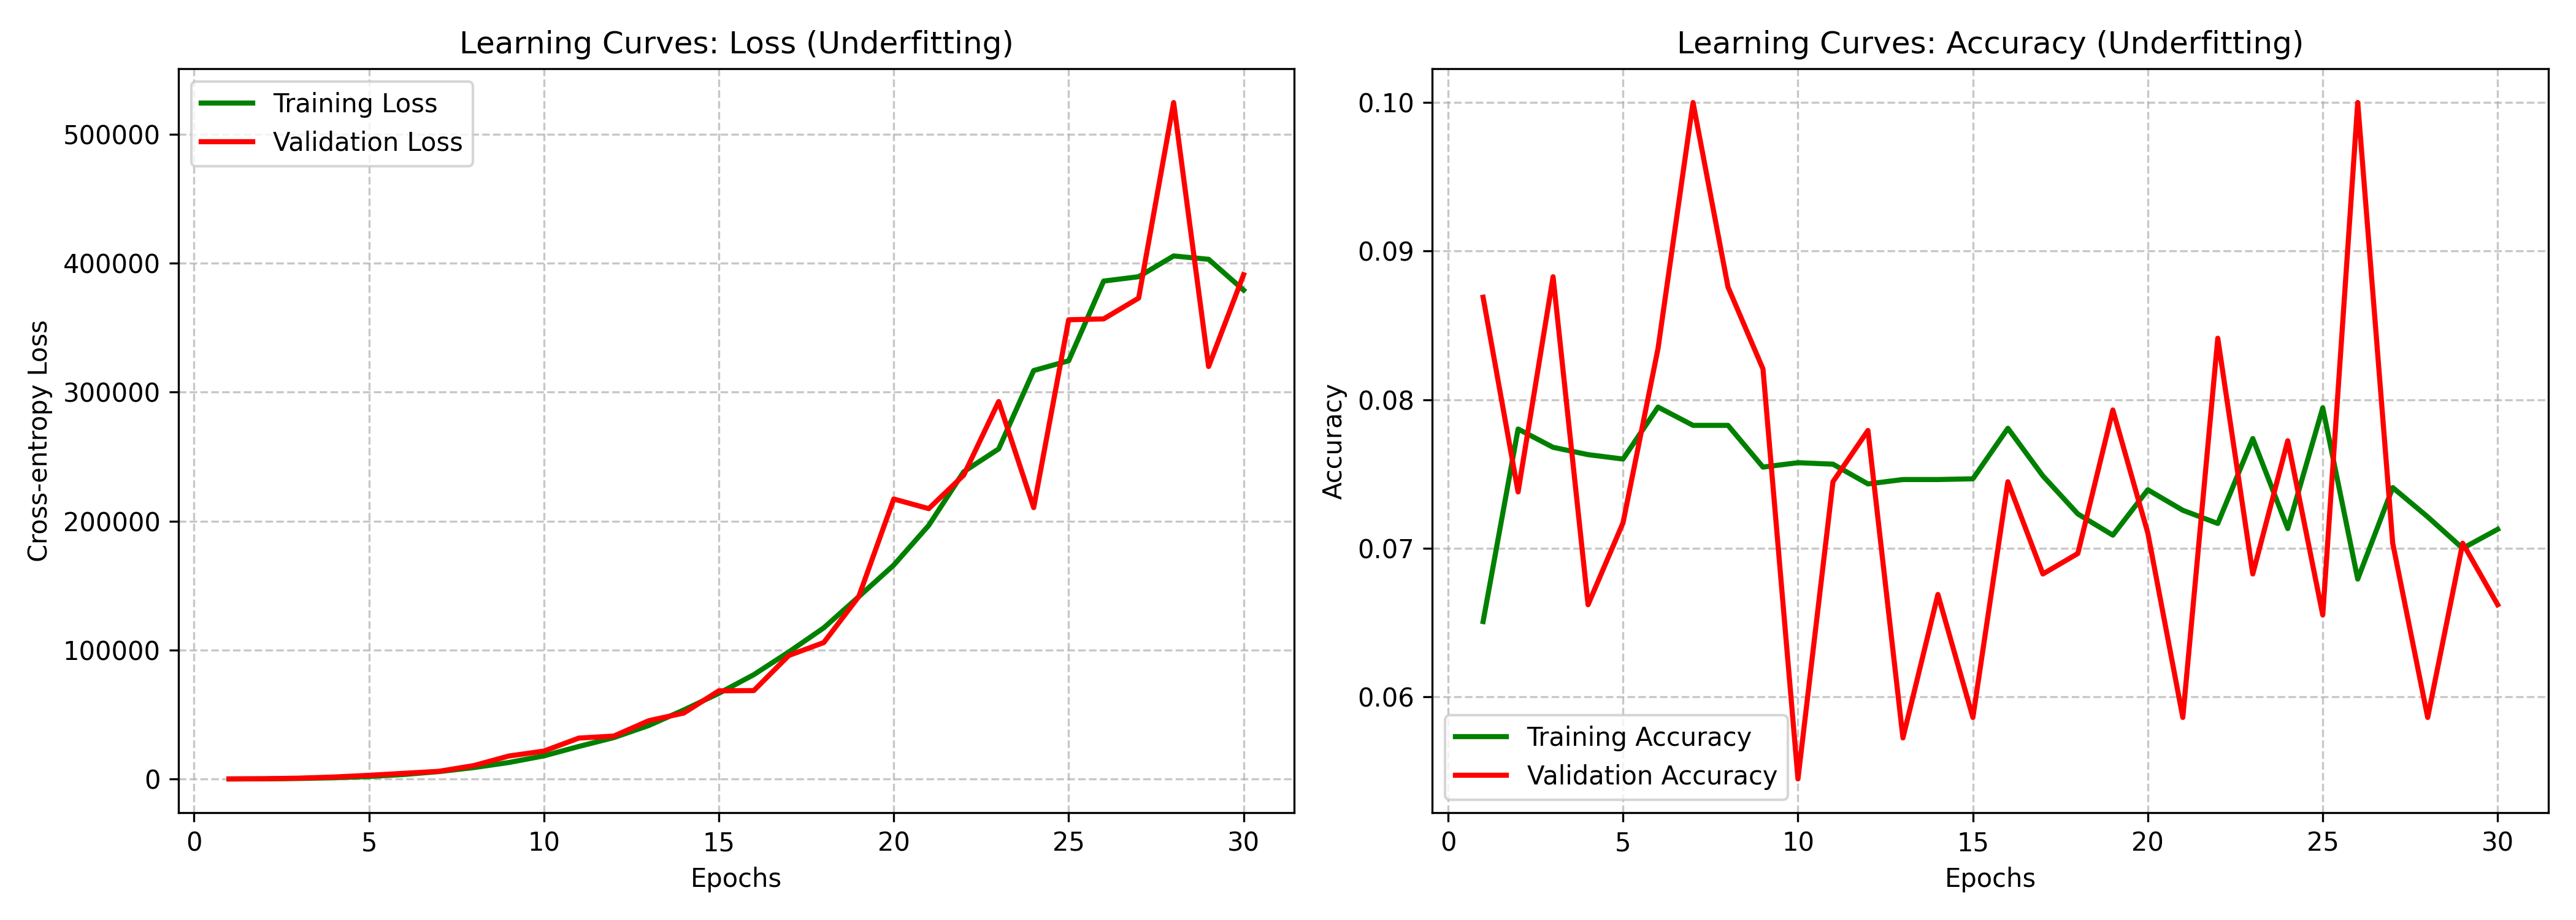
\includegraphics[width=0.95\textwidth]{01_underfit_plot.png}
\caption{Training and validation cross-entropy loss (left) and accuracy (right) for the underfitting model over 30 epochs.}
\label{fig:underfit}
\end{figure}

\subsubsection{Overfitting Scenario}
Figure~\ref{fig:overfit} illustrates that the unregularized 4-block CNN demonstrates textbook overfitting. Training loss decreases smoothly and monotonically from approximately 2.37 at epoch 1 to nearly 0.04 by epoch 20, while training accuracy climbs rapidly from 30\% to over 93\% by epoch 10 and plateaus at approximately 99\% for the remainder of training. In contrast, validation loss reaches its minimum of roughly 1.12 around epoch 6 and then diverges steadily upward to approximately 2.43--2.58 by epochs 28--30, indicating growing overconfidence on misclassified validation examples. Validation accuracy peaks near 70\% around epoch 16 and then stagnates and declines toward 65.5\% by epoch 30, resulting in a generalization gap of more than 30 percentage points.

\begin{figure}[htbp]
\centering
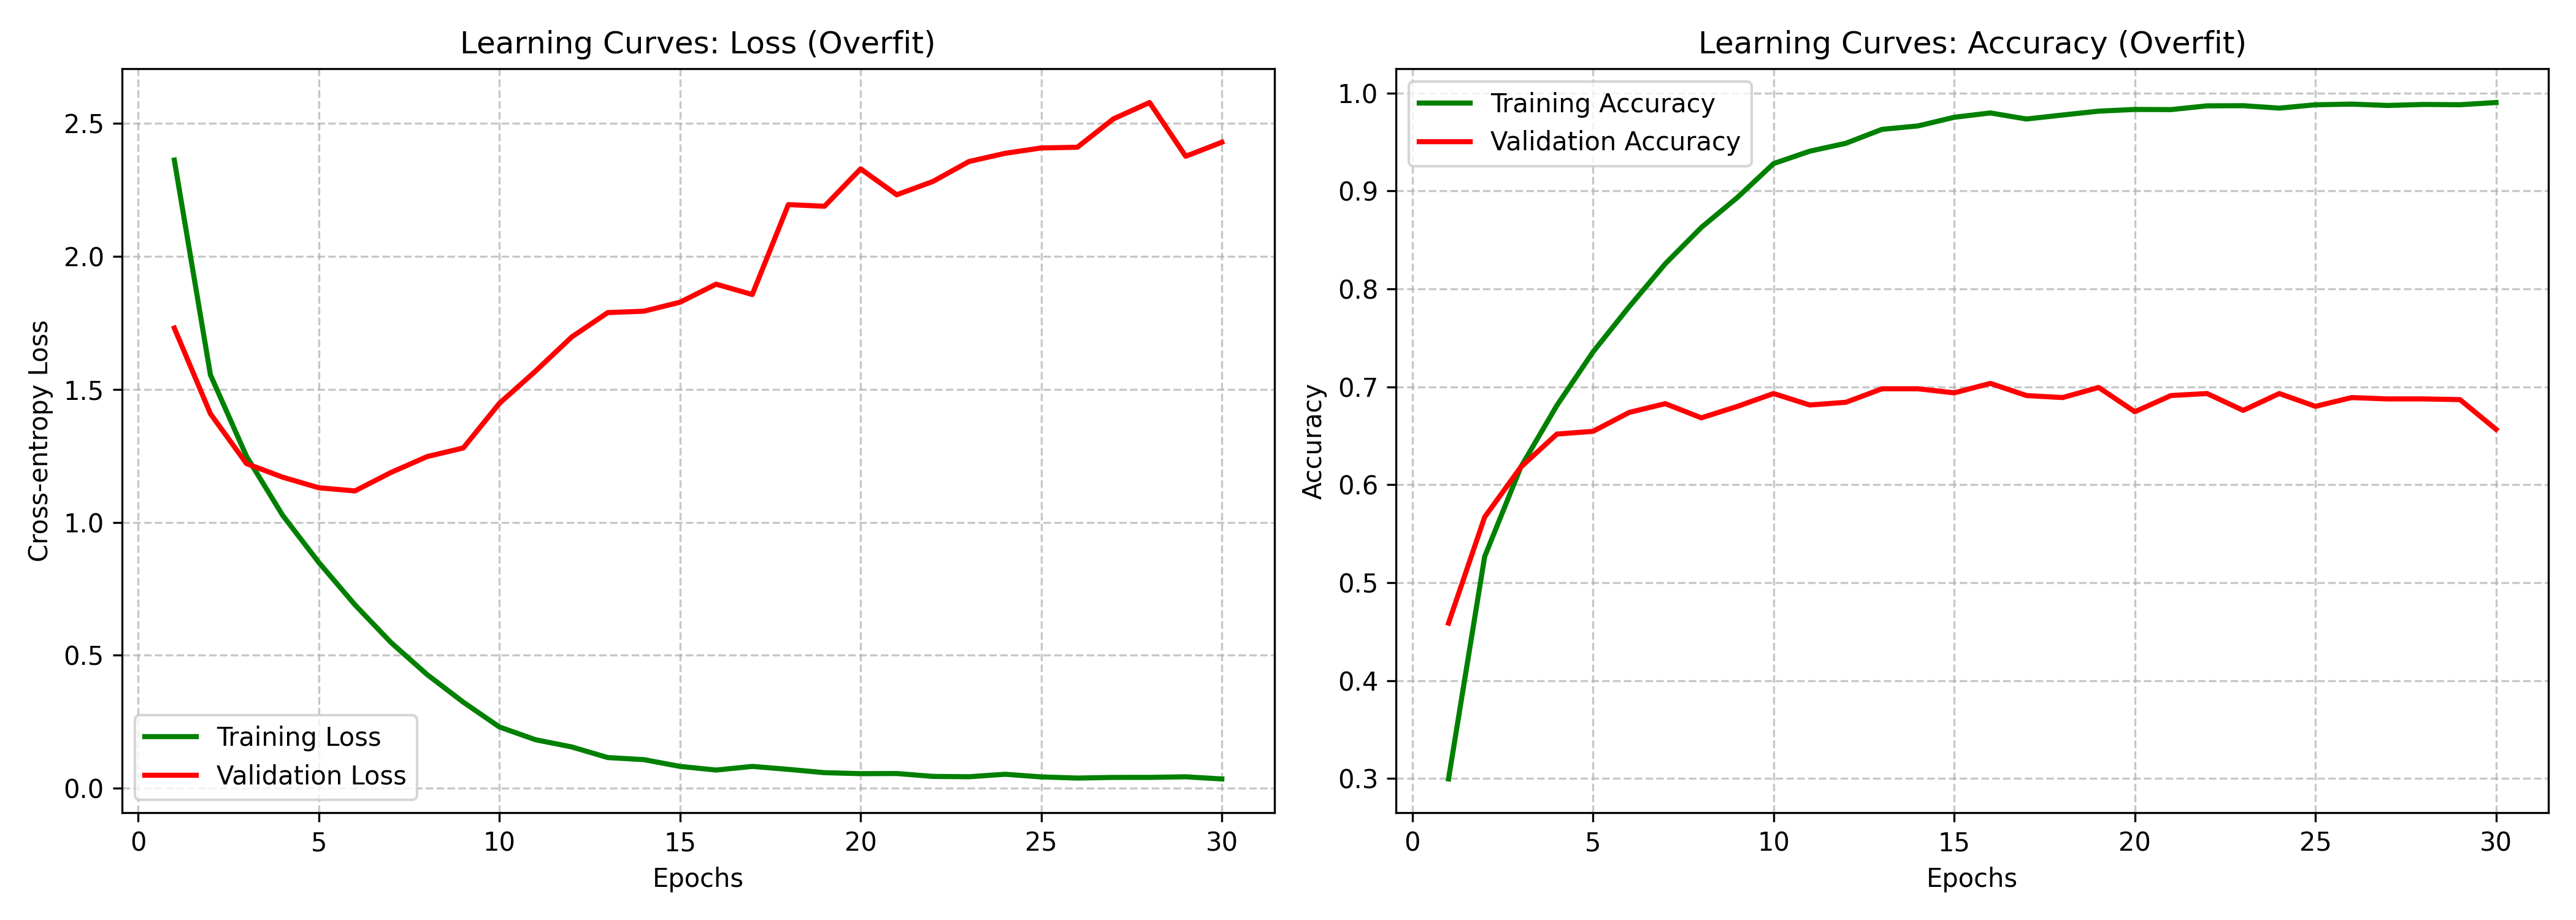
\includegraphics[width=0.95\textwidth]{01_overfit_plot.png}
\caption{Training and validation cross-entropy loss (left) and accuracy (right) for the overfitting model over 30 epochs.}
\label{fig:overfit}
\end{figure}

\subsubsection{Regularized Scenario}
As depicted in Figure~\ref{fig:regularized}, introducing regularization fundamentally transforms the learning dynamics. During the first 10 epochs, validation loss is slightly lower than training loss (and validation accuracy slightly higher than training accuracy) because data augmentation and dropout are active during training passes but disabled during validation. Both curves progress closely together throughout training, and the catastrophic validation-loss divergence observed in the overfitting model is entirely eliminated. Validation loss decreases from 2.19 at epoch 1 to a minimum of 1.1636 at epoch 26, where validation accuracy reaches its peak of 69.45\%. Because no further validation accuracy improvement exceeds $\text{min\_delta} = 10^{-3}$ over the subsequent 10 epochs, early stopping terminates training at epoch 36 and restores the optimal weights from epoch 26.

\begin{figure}[htbp]
\centering
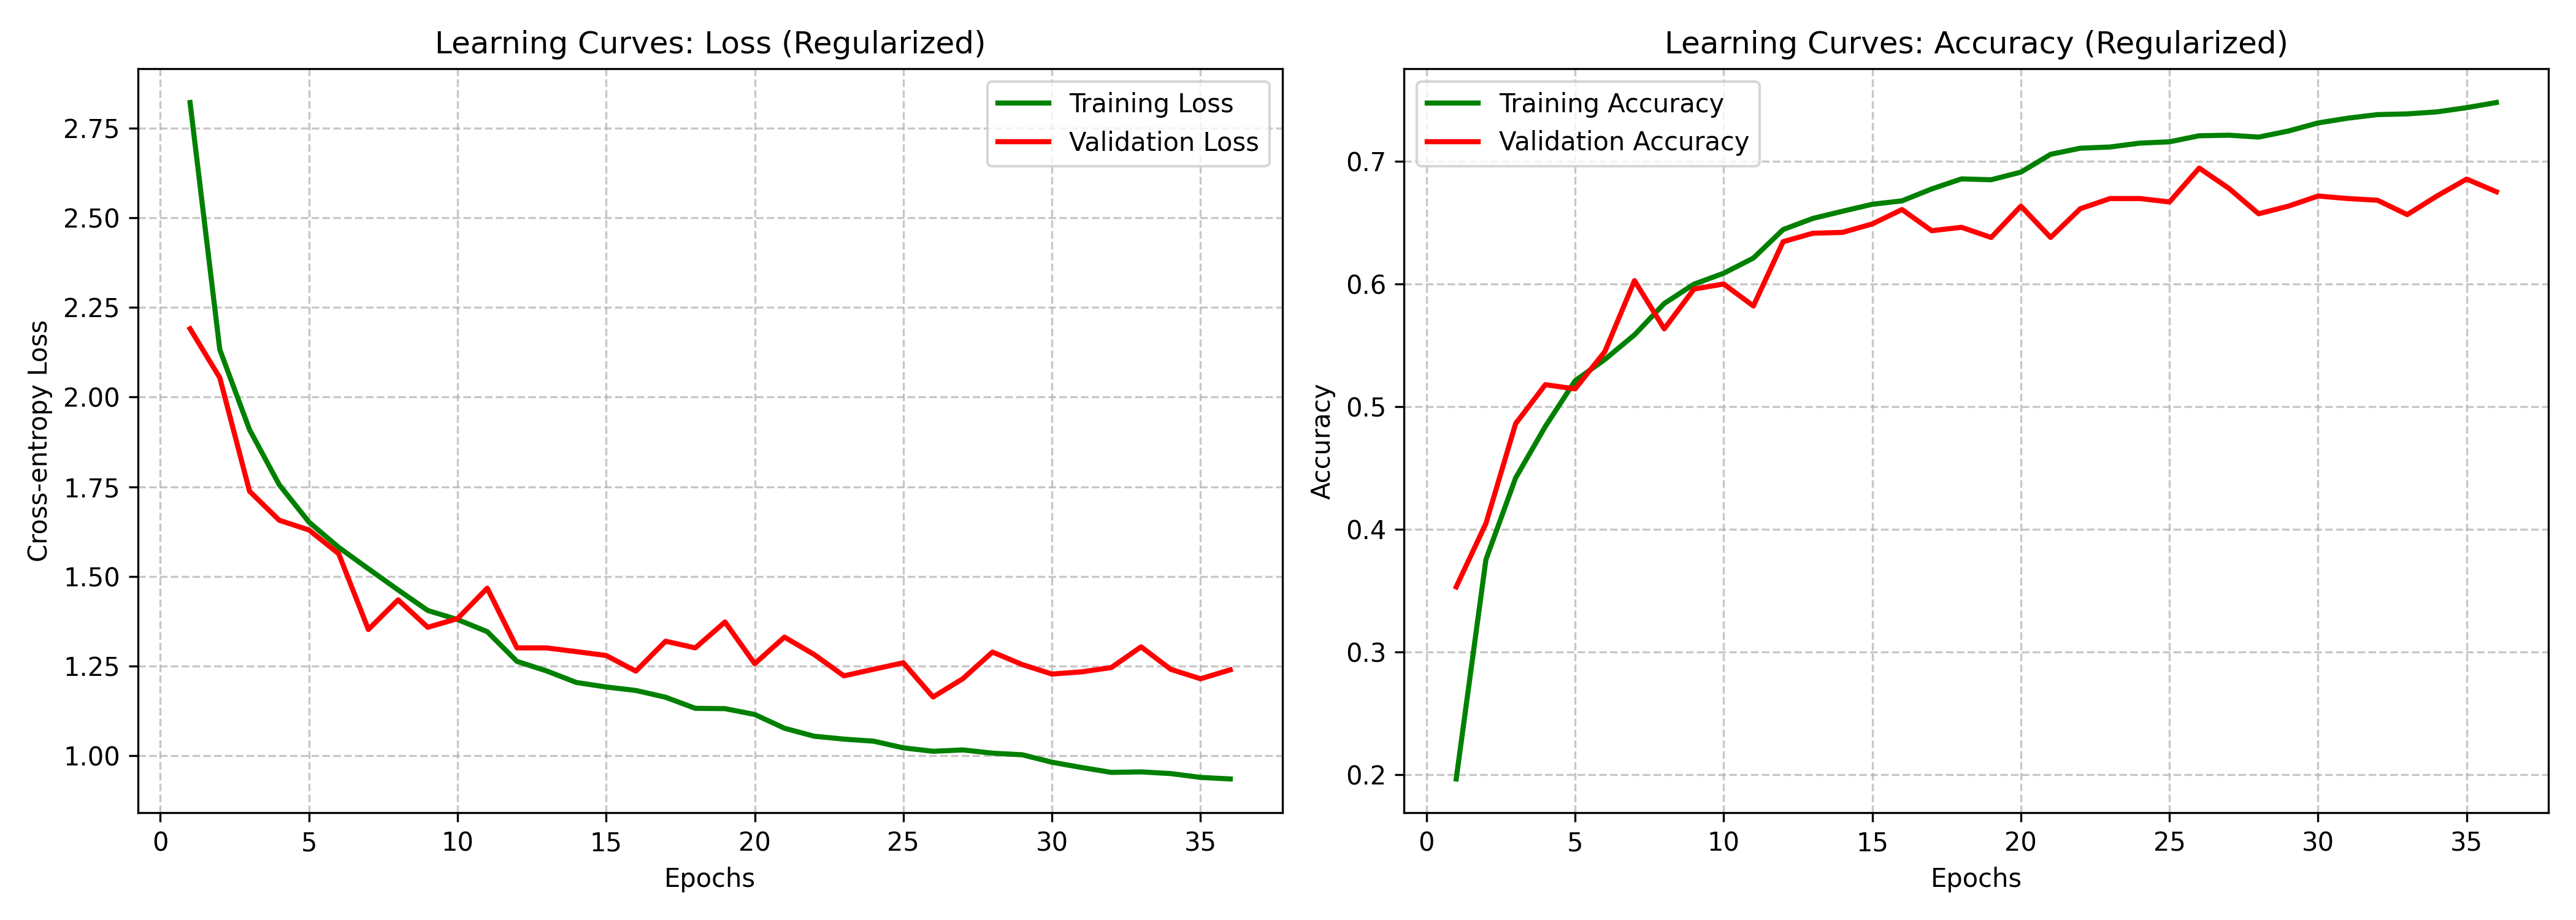
\includegraphics[width=0.95\textwidth]{01_regularized_plot.png}
\caption{Training and validation cross-entropy loss (left) and accuracy (right) for the regularized model (\texttt{01\_regularized\_model}), terminated by early stopping at epoch 36 with best weights restored from epoch 26.}
\label{fig:regularized}
\end{figure}

\subsection{Final Evaluation}

Because training-time metrics for the regularized model are computed with active dropout and data augmentation, they underestimate the model's true fit on unperturbed training images. To obtain an unbiased assessment of the generalization gap, the restored \texttt{01\_regularized\_model} (epoch 26 weights) was evaluated in pure inference mode across all three dataset splits. The results are summarized in Table~\ref{tab:split_eval}.

\begin{table}[htbp]
\centering
\caption{Inference-mode evaluation of \texttt{01\_regularized\_model} across all MAMe dataset splits.}
\label{tab:split_eval}
\begin{tabular}{@{}lccc@{}}
\toprule
\textbf{Dataset Split} & \textbf{Samples} & \textbf{Loss} & \textbf{Accuracy} \\
\midrule
Train (Inference) & 20,300 & 0.8726 & 77.12\% \\
Validation (Inference) & 1,450 & 1.1636 & 69.45\% \\
Test (Inference) & 15,657 & 1.1990 & 67.53\% \\
\midrule
\textbf{Test Balanced Accuracy (Macro Recall)} & 15,657 & --- & \textbf{68.53\%} \\
\bottomrule
\end{tabular}
\end{table}

In inference mode, the train--validation accuracy gap is reduced to 7.67 percentage points (77.12\% vs.\ 69.45\%), a substantial improvement over the $>30$ percentage-point gap of the unregularized model. Furthermore, the model generalizes robustly to the unseen test set, achieving 67.53\% overall accuracy (loss 1.1990) and 68.53\% balanced accuracy (macro-averaged recall). The small 0.92 percentage-point difference between balanced validation accuracy (69.45\%) and balanced test accuracy (68.53\%) confirms that hyperparameter tuning did not overfit to the validation set.

\section{Non-Standard CNN: Residual Network (ResNet)}
\label{sec:resnet}

\subsection{Model Architectures}

All ResNets are written with the Keras functional API. A $7 \times 7$ stride-2 convolution, batch normalization, ReLU and a $3 \times 3$ max-pooling form the stem. Stages of basic residual blocks (two $3 \times 3$ convolutions with batch normalization and a shortcut connection) with 64, 128, 256 and 512 filters follow; the first block of stages 2 to 4 downsamples with stride 2 and a $1 \times 1$ convolution on its shortcut. Global average pooling and a 29-way softmax layer terminate the network. Table~\ref{tab:resnet_architectures} summarizes the three configurations. Runs are numbered as in our log and were not performed in the order of the scenarios below. They were executed on one NVIDIA H100 GPU of MareNostrum 5.

\begin{table}[htbp]
\centering
\caption{Comparison of the three ResNet configurations evaluated on the MAMe dataset.}
\label{tab:resnet_architectures}
\small
\begin{tabular}{@{}llll@{}}
\toprule
\textbf{Component} & \textbf{Reduced (21)} & \textbf{Overfit (02)} & \textbf{Regularized (10)} \\
\midrule
Residual stages & 2 (64--128) & 4 (64--512) & 4 (64--512) \\
Blocks per stage & 1, 1 & 1, 1, 1, 1 & 1, 1, 1, 1 \\
Parameters & 319,133 & 4,929,309 & 4,929,309 \\
Residual-branch init. & Zero scale & Default & Default \\
Data augmentation & None & None & Flip, Rot(0.08), Zoom(0.1) \\
Optimizer & Adam & Adam & AdamW ($0.05$) \\
LR schedule, stopping & Fixed, 60 ep. & Fixed, 30 ep. & ReduceLR + EarlyStop \\
\bottomrule
\end{tabular}
\end{table}

\subsubsection{Underfitting Architecture}
Low capacity was sought by removing residual stages or narrowing the network. The retained model keeps the first two stages (64 and 128 filters), i.e.\ 319,133 parameters (6.5\% of the overfitting model), and initializes to zero the scale of the last batch normalization of each residual block (Goyal et al., 2017, who study SGD on ImageNet), so that the residual branch of every block initially outputs zero. Most narrower or shallower networks failed to train, learned slowly or overfitted (Section~\ref{sec:resnet_curves}).

\subsubsection{Overfitting Architecture}
The starting point is the ResNet-34 of the course (3, 4, 6 and 3 blocks per stage, 21,325,085 parameters). The overfitting model used in the rest of the study keeps its stem and widths with a single block per stage (4,929,309 parameters) and is trained for 30 epochs without augmentation or explicit regularization, which with 20,300 training images favors memorization.

\subsubsection{Regularized Architecture}
The regularized model keeps the backbone of the overfitting model and adds:
\begin{itemize}
    \item \textbf{Online Data Augmentation:} Horizontal flipping, rotations of up to $\pm 0.08$ turn ($\pm 29^\circ$, since the Keras factor is a fraction of $2\pi$) and random zooming of up to $10\%$, applied only during training.
    \item \textbf{Weight Decay:} AdamW with a decoupled weight decay of 0.05 replaces Adam.
    \item \textbf{Adaptive Optimization and Early Stopping:} \texttt{ReduceLROnPlateau} halves the learning rate (down to $10^{-6}$) when validation loss stagnates for 4 epochs, and \texttt{EarlyStopping} monitors validation accuracy with a patience of 10 epochs and restores the best weights (60 epochs at most).
\end{itemize}
A variant (run 23) adds \texttt{SpatialDropout2D} with a rate of 0.3 between the two convolutions of every residual block, the placement used by wide residual networks (Zagoruyko and Komodakis, 2016).

\subsection{Learning Curve Analysis}

\subsubsection{Underfitting Scenario}
\label{sec:resnet_curves}
We did not obtain a clean underfitting model. Networks of base width 8 and 16 (runs 03 and 04) stay at the loss of a uniform predictor, $\ln 29 = 3.367$, with a training accuracy of 0.03. These look like optimization failures rather than underfitting (the course attributes a loss that does not decrease to a bad initialization or learning rate), a cause we did not diagnose: the same code at a width of 32 learned in one run (run 05, from epoch 10) and not in another (run 14), and we did not vary the initialization (Keras default, Glorot; the course recommends He for ReLU) or the learning rate. Two stages without the zero initialization (run 17) collapse to chance, and a single stage (run 22) diverges. The other attempts learned but did not underfit: widths 24 and 32 with augmentation overfit (runs 06 and 15, training accuracy 69\% and 83\%), three stages with the zero initialization overfit (run 19, 96\% after 100 epochs), three stages without it learn poorly (runs 16 and 18, 43\% after 30 epochs and 38\% after 100), and a width of 16 with it stays at chance (run 20). The retained model (run 21, Figure~\ref{fig:resnet_underfit}) does learn, but slowly: after 60 epochs its training accuracy is 54.8\% and still rises by about 0.24 point per epoch, so it cannot be distinguished from a model that has not finished converging. Narrowing the same two-stage network to a width of 48 (run 42, 182,525 parameters) does not give an underfit either: its training accuracy reaches 73.4\% after 60 epochs, still rising, and a width of 32 (run 43) diverges (loss above 700).

The logged validation accuracy of run 21 (31.8\%) is probably misleading: the moving averages of the batch normalization layers lag behind the weights (batch statistics are used in training, running averages in inference). After recomputing them from 32 batches of training images, its validation accuracy is 53.3\% (loss 1.65), close to the training accuracy of 58.1\% measured the same way (CPU, single run, approximate recalibration). The other logged validation curves are probably affected as well.

Table~\ref{tab:levers} lists the levers applied to the overfitting ResNet. Several lower the training accuracy (dropout 0.5 to 0.9: 0.69 to 0.77 and strong augmentation: 0.74, both measured with the perturbation active; weight decay 5.0: 0.63) and in most cases it keeps rising, while label smoothing 0.5 and weight decay 1.0 do not lower it at all (0.996 and 0.98). Only the weight decay of 5.0 reaches a plateau (runs 31 and 33), at a training accuracy of 63\%; the validation accuracy of run 31 is 33\%, so the gap is not small and it is not an underfit in the sense of the course (both remain high, small gap), even though its logged validation accuracy is probably lowered by the batch normalization lag. Reducing the input resolution lowers the validation accuracy (58\% to 42\%) more than the training accuracy (100\% to 92\%), consistent with fine details being decisive on MAMe (Par\'es et al., 2022).

\begin{table}[htbp]
\centering
\caption{Levers applied to the overfitting ResNet (30 epochs, one run each; runs 42 and 43: 60 epochs, built on run 21). Last-epoch training accuracy, validation accuracy averaged over the last 10 epochs, and trend of the training accuracy, from a line fitted to the last 10 epochs: saturated above 0.97 with a slope below 0.3 point per epoch, plateau below 0.1 point per epoch, noisy when the residual standard deviation exceeds 1 point, rising otherwise.}
\label{tab:levers}
\footnotesize
\begin{tabular}{@{}>{\raggedright\arraybackslash}p{5.1cm}>{\raggedright\arraybackslash}p{2.9cm}>{\raggedright\arraybackslash}p{2.9cm}>{\raggedright\arraybackslash}p{2.6cm}@{}}
\toprule
\textbf{Lever (runs)} & \textbf{Train} & \textbf{Val} & \textbf{Train trend} \\
\midrule
SpatialDropout 0.5 / 0.7 / 0.9 (24--26) & 0.77 / 0.73 / 0.69 & 0.53 / 0.47 / 0.45 & rising \\
Label smoothing 0.5 / 0.9 (27, 28) & 1.00 / 0.47 & 0.61 / 0.21 & saturated / noisy \\
Strong augmentation (29) & 0.74 & 0.42 & rising \\
AdamW, weight decay 1.0 / 5.0 (30, 31) & 0.98 / 0.63 & 0.39 / 0.33 & rising / plateau \\
Dropout 0.7 after pooling (32) & 0.95 & 0.56 & rising \\
BN momentum 0.9, with weight decay 5.0 / alone / with spatial dropout 0.9 (33--35) & 0.63 / 1.00 / 0.68 & 0.36 / 0.65 / 0.50 & plateau / saturated / rising \\
Input average pooling $4 / 8 / 16 / 32$ (36--39) & 1.00 / 0.98 / 0.95 / 0.92 & 0.58 / 0.54 / 0.48 / 0.42 & saturated / saturated / rising / rising \\
Stem kernel $3 \times 3$ / $1 \times 1$ (40, 41) & 0.98 / 0.99 & 0.58 / 0.64 & saturated \\
Width 48 / 32, 2 stages (42, 43) & 0.73 / 0.05 & 0.42 / 0.06 & rising / diverges \\
\bottomrule
\end{tabular}
\end{table}

\begin{figure}[htbp]
\centering
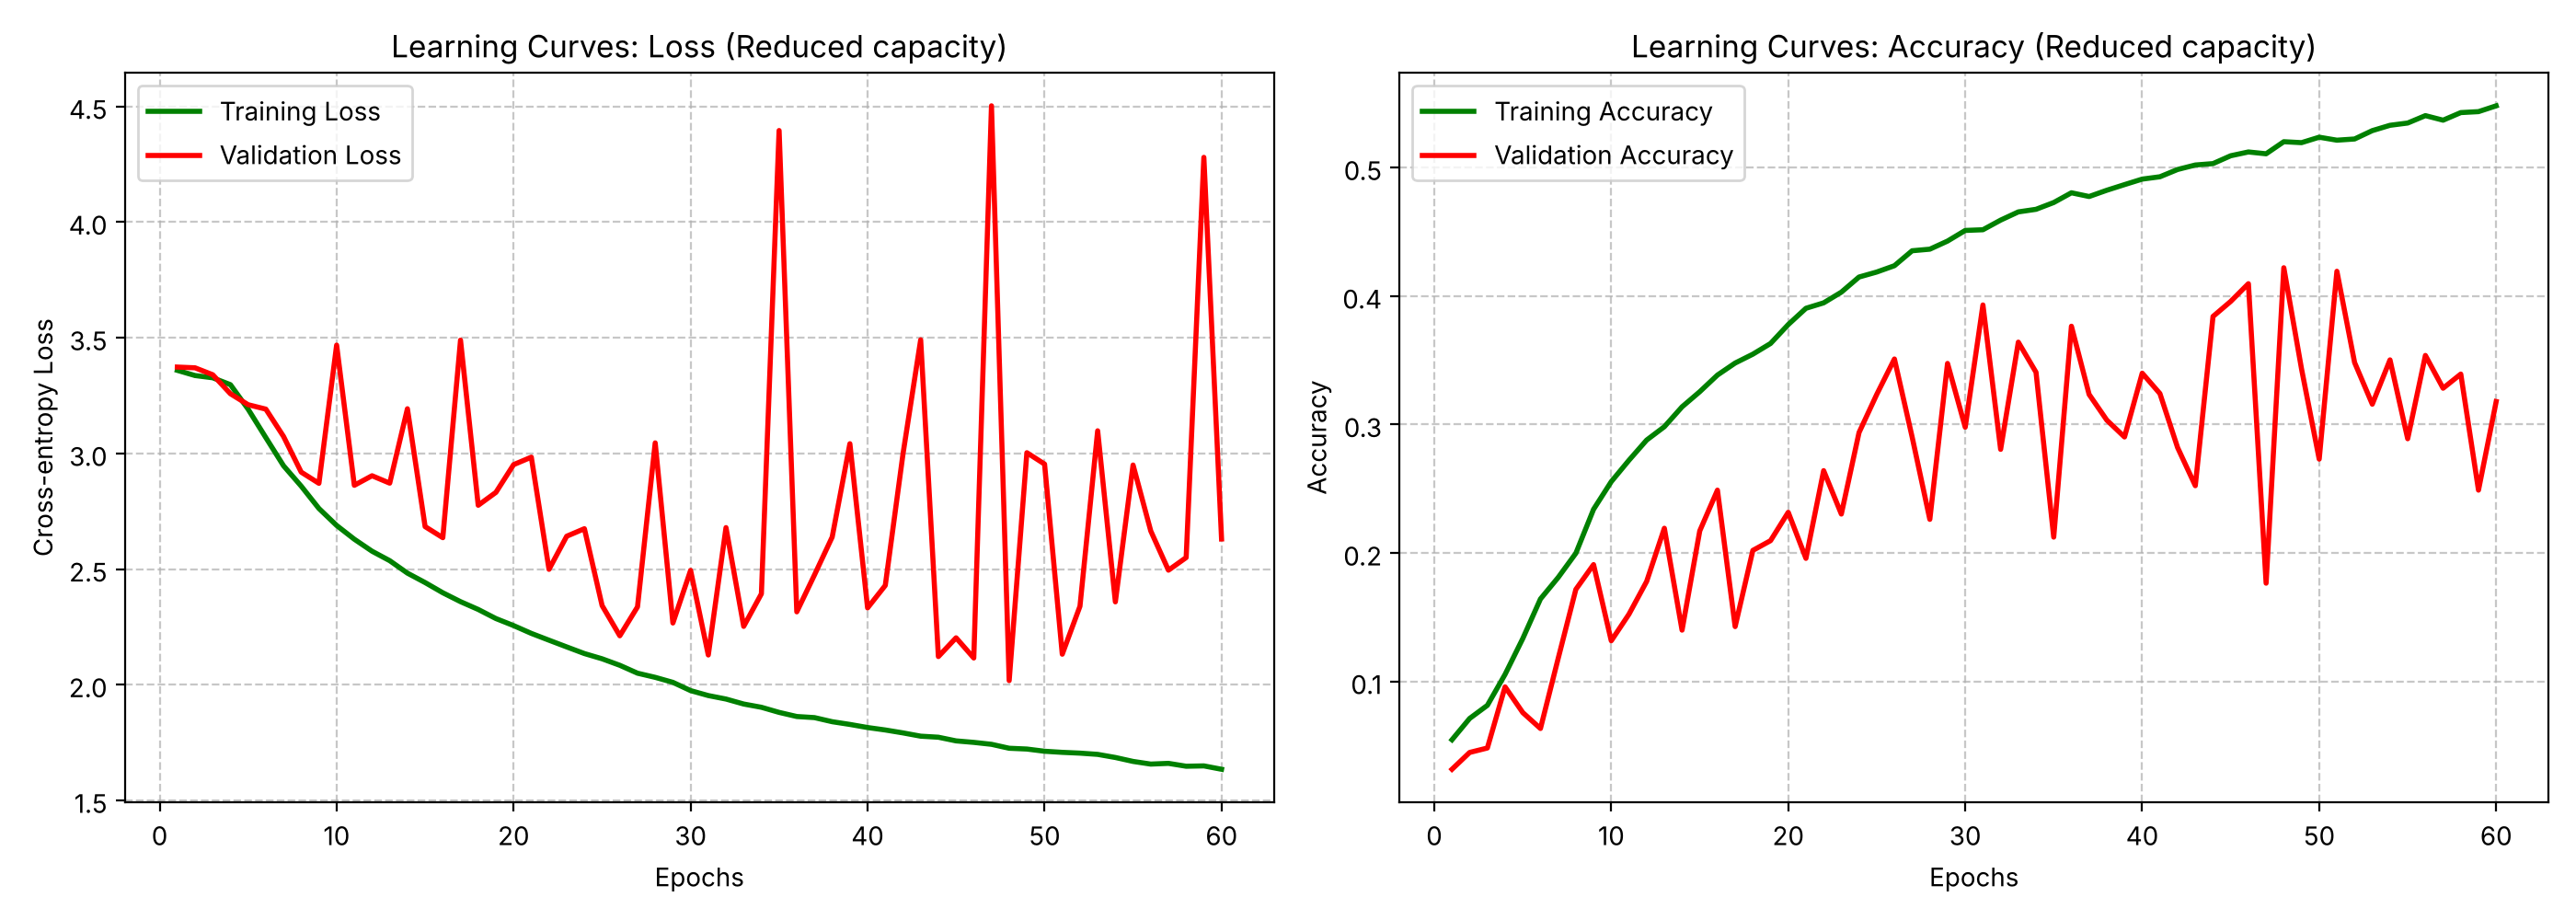
\includegraphics[width=0.8\textwidth]{21_reduced_capacity_plot.png}
\caption{Training and validation cross-entropy loss (left) and accuracy (right) for the reduced ResNet (run 21) over 60 epochs. The validation curve uses the batch normalization moving averages of each epoch.}
\label{fig:resnet_underfit}
\end{figure}

\subsubsection{Overfitting Scenario}
Figure~\ref{fig:resnet_overfit} shows that the single-block ResNet memorizes the training set. Its training accuracy exceeds 95\% from epoch 18 and reaches 99.2\% at epoch 30 (loss 0.04), while the validation accuracy oscillates between 46\% and 70\% over the last 10 epochs (average 59.4\%) and the validation loss does not go below 1.165. The gap between the logged training and validation accuracy is about 40 percentage points. The ResNet-34 of the course behaves the same way: 95.1\% training accuracy against 55.2\% validation accuracy (average over the last 10 epochs).

\begin{figure}[htbp]
\centering
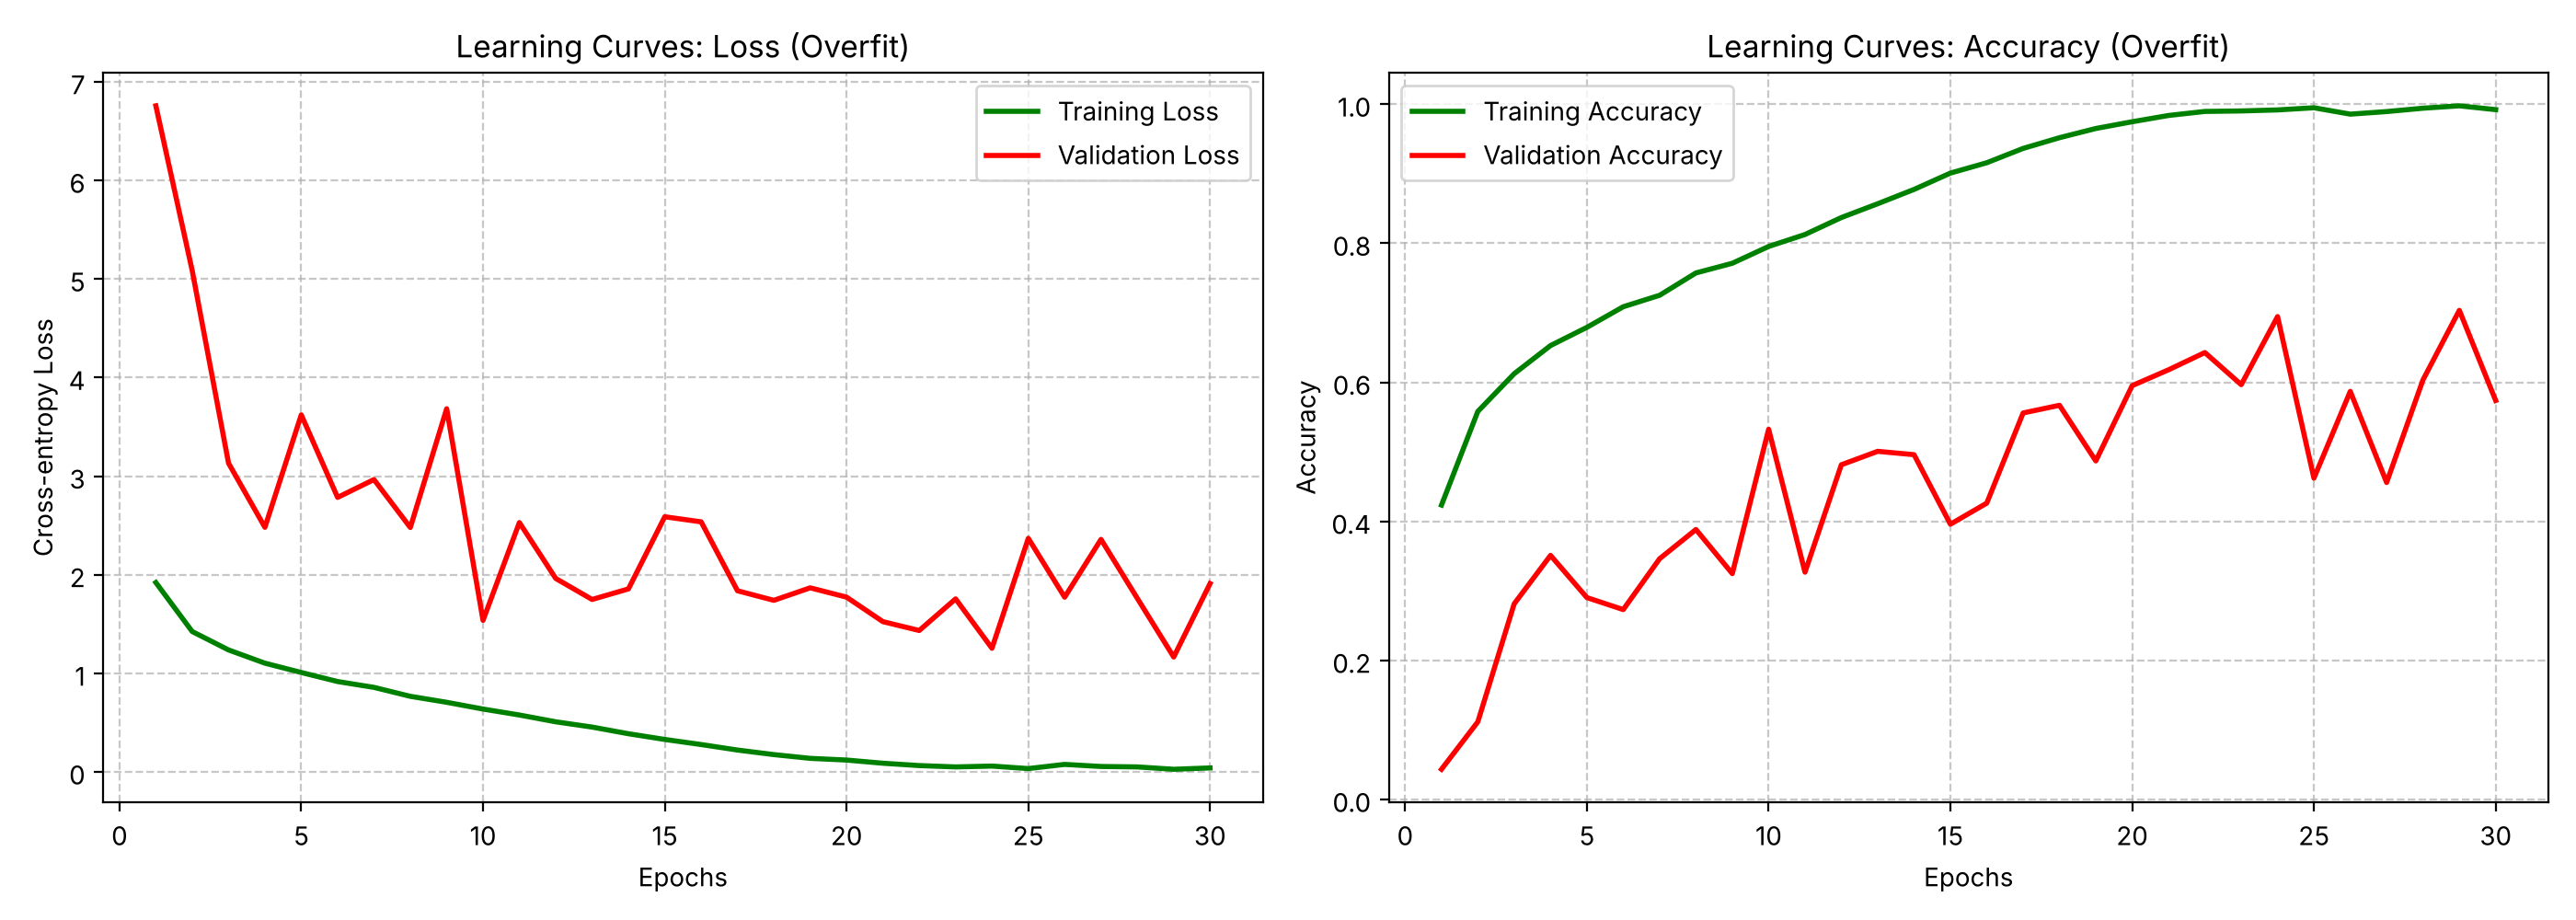
\includegraphics[width=0.8\textwidth]{02_overfit_plot.png}
\caption{Training and validation cross-entropy loss (left) and accuracy (right) for the overfitting ResNet (run 02) over 30 epochs.}
\label{fig:resnet_overfit}
\end{figure}

\subsubsection{Regularized Scenario}
Augmentation alone (run 07) and with decoupled weight decay (run 08), 30 epochs each, did not stabilize the validation accuracy (49\% and 43\% over the last 10 epochs, training still rising); adding learning-rate decay, early stopping and a budget of up to 60 epochs did (runs 09 and 10, Figure~\ref{fig:resnet_regularized}), without separating the effect of these three changes. Run 10 repeats the code of run 09, whose best validation accuracy is 70.7\%; it is the better of the two runs, so its figures include a selection bias of the order of the 2-point difference. Validation loss reaches its minimum of 0.926 at epoch 34 and validation accuracy peaks at 72.8\% at epoch 44; early stopping ends training at epoch 54 and restores the weights of epoch 44. Smaller initial learning rates did not improve on run 09 (best validation accuracy 69.5\% and 63.1\% for $3 \times 10^{-4}$ and $10^{-4}$, runs 11 and 12, the latter stopped at epoch 26), although a single run each cannot separate 69.5\% from 70.7\%. The variant with spatial dropout (run 23) stops at epoch 41 and restores epoch 31: its training and validation curves stay closer, but its validation accuracy is 67.7\%, about 5 points lower.

\begin{figure}[htbp]
\centering
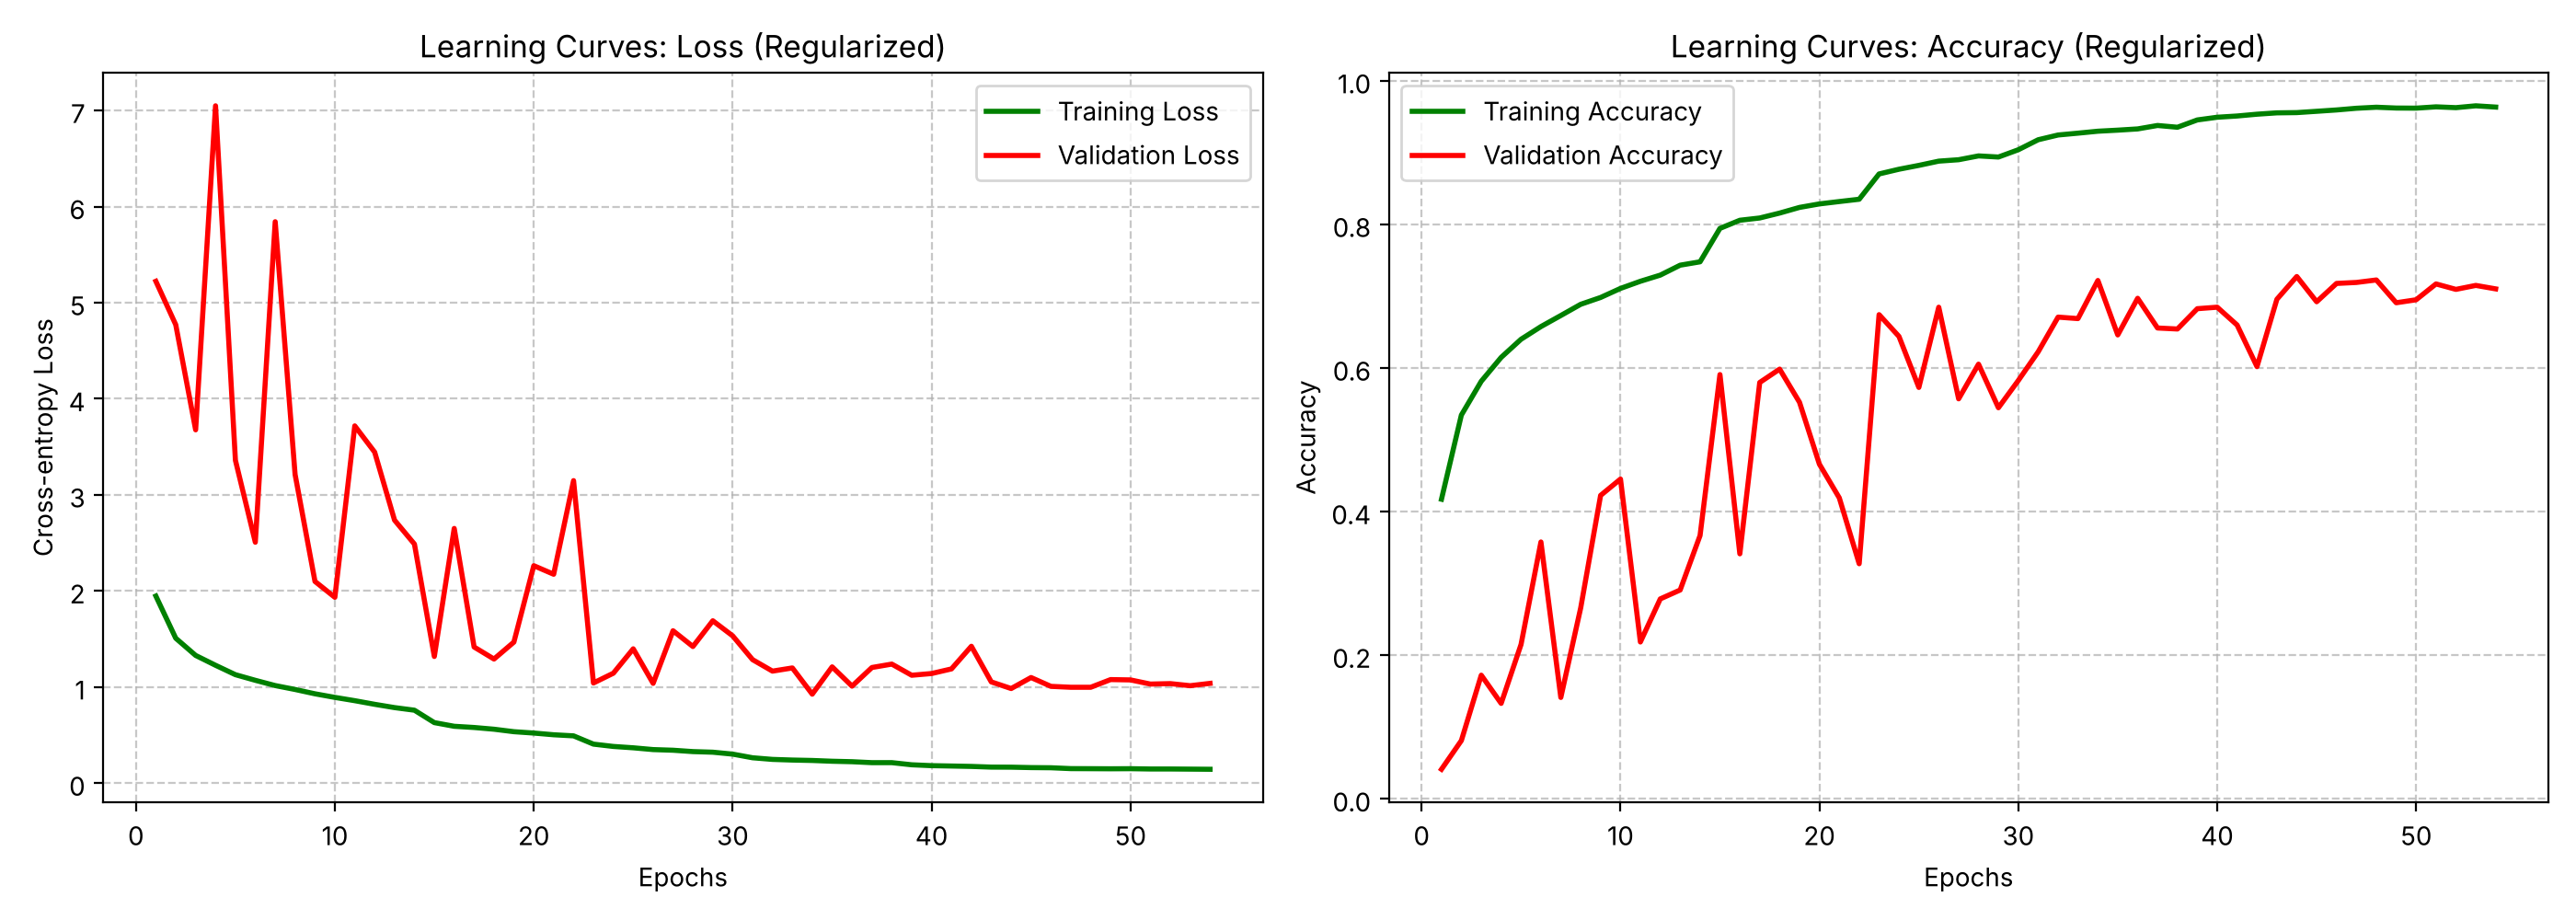
\includegraphics[width=0.8\textwidth]{10_regularized_plot.png}
\caption{Training and validation cross-entropy loss (left) and accuracy (right) for the regularized ResNet (run 10), terminated by early stopping at epoch 54 with best weights restored from epoch 44.}
\label{fig:resnet_regularized}
\end{figure}

\subsection{Final Evaluation}

The logged training metrics are computed in training mode and differ from a pure inference pass. The restored models (epoch 44 for run 10, epoch 31 for run 23) were therefore evaluated in inference mode across all three dataset splits. The results are summarized in Table~\ref{tab:resnet_split_eval}.

\begin{table}[htbp]
\centering
\caption{Inference-mode evaluation of the regularized ResNet (run 10) and of the variant with spatial dropout (run 23) across all MAMe dataset splits.}
\label{tab:resnet_split_eval}
\begin{tabular}{@{}lccccc@{}}
\toprule
 & & \multicolumn{2}{c}{\textbf{Run 10}} & \multicolumn{2}{c}{\textbf{Run 23}} \\
\cmidrule(lr){3-4}\cmidrule(lr){5-6}
\textbf{Dataset Split} & \textbf{Samples} & \textbf{Loss} & \textbf{Accuracy} & \textbf{Loss} & \textbf{Accuracy} \\
\midrule
Train (Inference) & 20,300 & 0.3549 & 88.49\% & 0.8426 & 73.01\% \\
Validation (Inference) & 1,450 & 0.9851 & 72.76\% & 1.0349 & 67.66\% \\
Test (Inference) & 15,657 & 1.0183 & 72.34\% & 1.0727 & 66.76\% \\
\midrule
\textbf{Test Balanced Accuracy} & 15,657 & --- & \textbf{73.27\%} & --- & \textbf{68.17\%} \\
\bottomrule
\end{tabular}
\end{table}

In inference mode, the train--validation accuracy gap is 15.7 percentage points for run 10 (88.49\% vs.\ 72.76\%) and 5.4 points for run 23 (73.01\% vs.\ 67.66\%): spatial dropout reduces the gap but costs about 5 points of accuracy on both validation and test sets. Run 10 reaches 72.34\% test accuracy (loss 1.0183) and 73.27\% balanced accuracy. The drop from validation to test accuracy is only 0.4 points (0.9 for run 23), so there is no sign that selecting the best epoch on the validation set overfit it (the drop is smaller than the validation standard error of about 1.2 points). We retain run 10 as the regularized ResNet. This choice was made after both models had been evaluated on the test set; the validation accuracy alone gives the same ordering.

\section{Comparison and Summary}
\label{sec:summary}

\textbf{Standard CNN.} Through a controlled progression from underfitting to overfitting and targeted regularization, our standard 4-block CNN trained from scratch achieves 69.45\% validation accuracy, 67.53\% test accuracy, and 68.53\% test balanced accuracy across 29 artwork media. Combining online data augmentation, L2 weight decay, spatial and standard dropout, adaptive learning rate scheduling, and early stopping effectively eliminates validation-loss divergence and narrows the generalization gap from over 30 percentage points to 7.67 percentage points without modifying the core convolutional backbone.

\textbf{ResNet.} The ResNet-34 of the course overfits on MAMe, as expected for 21 million parameters and 20,300 images. Reducing the network did not give a clean underfitting regime: the smallest networks fail to train and the intermediate ones converge slowly. Learning-rate scheduling with early stopping, together with data augmentation and weight decay, gives the regularized ResNet (72.34\% test accuracy, 73.27\% balanced accuracy, train--validation gap of 15.7 points). Adding spatial dropout reduces the gap to 5.4 points but lowers the test accuracy to 66.76\%.

\textbf{Comparison.} Table~\ref{tab:comparison} puts the two families side by side. Both have about 5 million parameters, but 91.4\% of the standard CNN parameters lie in one dense layer, whereas the ResNet ends with global average pooling. The regularized ResNet has the highest test accuracy and balanced accuracy of this report, 4.8 and 4.7 points above the regularized standard CNN, but also the largest train--validation gap (15.7 points against 7.67). The ResNet with spatial dropout is close to the standard CNN (0.8 points lower in test accuracy). Each reported model comes from one training run, and two runs of the same ResNet code (09 and 10) differ by about 2 points of validation accuracy; run 10 is the better of the two. The ResNet also differs from the standard CNN by batch normalization, AdamW, up to 60 epochs and many more tuning runs, so no ablation attributes its advantage to the dense layer alone.

\begin{table}[htbp]
\centering
\caption{Standard CNN and ResNet side by side (inference mode, restored best epoch).}
\label{tab:comparison}
\small
\begin{tabular}{@{}lcccc@{}}
\toprule
\textbf{Model} & \textbf{Parameters} & \textbf{Val acc.} & \textbf{Test acc.} & \textbf{Test bal. acc.} \\
\midrule
Standard CNN, regularized & 4,590,429 & 69.45\% & 67.53\% & 68.53\% \\
ResNet, regularized (run 10) & 4,929,309 & 72.76\% & 72.34\% & 73.27\% \\
ResNet, spatial dropout (run 23) & 4,929,309 & 67.66\% & 66.76\% & 68.17\% \\
\bottomrule
\end{tabular}
\end{table}

\textbf{Limitations.} Essentially one run per configuration, a validation set of 1,450 images (standard error of about 1.2 points), and no clean underfitting model for either family.

\end{document}
